\documentclass[a4paper,11pt]{report}
\usepackage{chuan_math_gkt}
\usetikzlibrary{angles,quotes,intersections,patterns,decorations.pathreplacing}
\chuanexamsetup

\begin{document}
\examfontsize

\examsecret{绝密$\bigstar$启用前}

\examtitle{2020年普通高等学校招生全国统一考试（新课标II卷文科）}{数\quad 学}

\noticetitle
\begin{examnotice}
\item 答卷前，考生务必将自己的姓名、准考证号填写在答题卡上。
\item 回答选择题时，选出每小题的答案后，用铅笔把答题卡上对应题目的答案标号涂黑。如需改动，用橡皮擦干净后，再选涂其他答案标号。回答非选择题时，将答案写在答题卡上。写在本试卷上无效。
\item 考试结束后，将本试卷和答题卡一并交回。
\end{examnotice}
\examsection{一、选择题：本题共12小题，每小题5分，共60分。在每小题给出的四个选项中，只有一项是符合题目要求的。}
\begin{examquestions}

\item 已知集合\emph{A}=\{\emph{x}\textbar\textbar{}\emph{x}\textbar<3，\emph{x}\ensuremath{\in}\emph{Z}\}，\emph{B}=\{\emph{x}\textbar\textbar{}\emph{x}\textbar>1，\emph{x}\ensuremath{\in}\emph{Z}\}，则\emph{A}\ensuremath{\cap}\emph{B}=

\fourchoices{$\varnothing$}{\{--3，--2，2，3）}{\{--2，0，2\}}{\{--2，2\}}

\item （1--i）\textsuperscript{4}=

A --4 B. 4

C. --4\emph{i} D. 4\emph{i}

\item 如图，将钢琴上的12个键依次记为\emph{a}$_{1}$，\emph{a}$_{2}$，\ensuremath{\ldots}，\emph{a}\textsubscript{12}.设1\ensuremath{\leq}\emph{i}<{}\emph{j}<{}\emph{k}\ensuremath{\leq}12．若\emph{k}--\emph{j}=3且\emph{j}--\emph{i}=4，则称\emph{$a_{i}$}，\emph{$a_{j}$}，\emph{$a_{k}$}为原位大三和弦；若\emph{k}--\emph{j}=4且\emph{j}--\emph{i}=3，则称\emph{$a_{i}$}，\emph{$a_{j}$}，\emph{$a_{k}$}为原位小三和弦．用这12个键可以构成的原位大三和弦与原位小三和弦的个数之和为

\begin{tightcenter}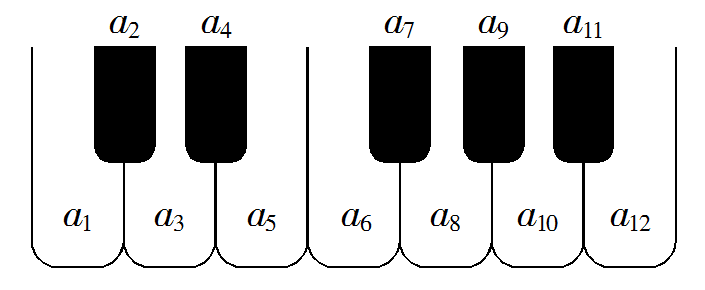
\includegraphics[width=2.95833in,height=1.21875in]{figures/2020_xkb2_wen_image3.png}\end{tightcenter}

\emph{A.} 5 \emph{B.} 8 \emph{C.} 10 \emph{D.} 15

\item 在新冠肺炎疫情防控期间，某超市开通网上销售业务，每天能完成1200份订单的配货，由于订单量大幅增加，导致订单积压.为解决困难，许多志愿者踊跃报名参加配货工作.已知该超市某日积压500份订单未配货，预计第二天的新订单超过1600份的概率为0.05，志愿者每人每天能完成50份订单的配货，为使第二天完成积压订单及当日订单的配货的概率不小于0.95，则至少需要志愿者

\fourchoices{10名}{18名}{24名}{32名}

\item 已知单位向量\emph{{a}}，\emph{{b}}夹角为60°，则在下列向量中，与\emph{{b}}垂直的是

\fourchoices{\emph{{a}}+2\emph{{b}}}{2\emph{{a}}+\emph{{b}}}{\emph{{a}}--2\emph{{b}}}{2\emph{{a}}--\emph{{b}}}

\item 记\emph{$S_{n}$}为等比数列\{\emph{$a_{n}$}\}的前\emph{n}项和．若\emph{a}\textsubscript{5}--\emph{a}$_{3}$=12，\emph{a}\textsubscript{6}--\emph{a}\textsubscript{4}=24，则$\dfrac{S_{n}}{a_{n}}$=

\emph{{A.}} 2\emph{\textsuperscript{n}}--1 \emph{{B.}}
2--2\textsuperscript{1--\emph{n}} \emph{{C.}}
2--2\textsuperscript{\emph{n}--1} \emph{{D.}}
2\textsuperscript{1--\emph{n}}--1

\item 执行右面的程序框图，若输入的\emph{k}=0，\emph{a}=0，则输出的\emph{k}为

\begin{tightcenter}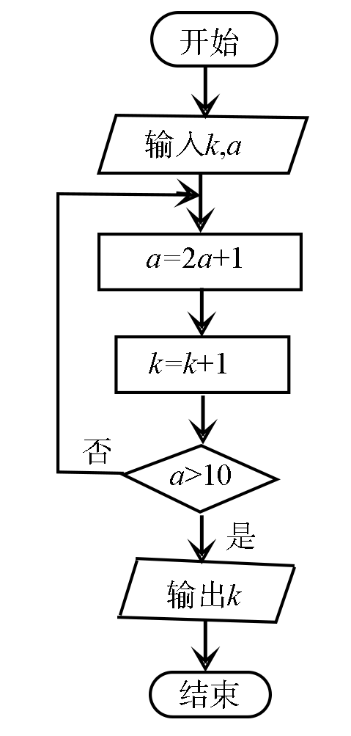
\includegraphics[width=1.59375in,height=3.33333in]{figures/2020_xkb2_wen_image6.png}\end{tightcenter}

\fourchoices{2}{3}{4}{5}

\item 若过点（2，1）的圆与两坐标轴都相切，则圆心到直线$2x-y-3=0$的距离为

\onechoices{$\dfrac{\sqrt{5}}{5}$}{$\dfrac{2\sqrt{5}}{5}$}{$\dfrac{3\sqrt{5}}{5}$}{$\dfrac{4\sqrt{5}}{5}$}

\item 设$O$为坐标原点，直线$x=a$与双曲线$C:\dfrac{x^{2}}{a^{2}}-\dfrac{y^{2}}{b^{2}}=1(a>0,b>0)$两条渐近线分别交于$D,E$两点，若$\ensuremath{\triangle}ODE$的面积为8，则$C$的焦距的最小值为

\fourchoices{4}{8}{16}{32}

\item 设函数$f(x)=x^{3}-\dfrac{1}{x^{3}}$,则$f(x)$

\fourchoices{是奇函数，且在(0,+∞)单调递增}{是奇函数，且在(0,+∞)单调递减}{是偶函数，且在(0,+∞)单调递增}{是偶函数，且在(0,+∞)单调递减}

\item 已知\ensuremath{\triangle}\emph{ABC}是面积为$\dfrac{9\sqrt{3}}{4}$的等边三角形，且其顶点都在球\emph{O}的球面上.若球\emph{O}的表面积为16\emph{π}，则\emph{O}到平面\emph{ABC}的距离为

\onechoices{$\sqrt{3}$}{$\dfrac{3}{2}$}{1}{$\dfrac{\sqrt{3}}{2}$}

\item 若$2^{x}-2^{y}<3^{-x}-3^{-y}$，则

\fourchoices{$\ln(y-x+1)>0$}{$\ln(y-x+1)<0$}{$\ln|x-y|>0$}{$\ln|x-y|<0$}

\item 若$sinx=-\dfrac{2}{3}$，则$cos2x=$\blank．

\item 记$S_{n}$为等差数列$\{a_{n}\}$的前\emph{n}项和．若$a_{1}=-2,a_{2}+a_{6}=2$，则$S_{10}=$\blank．

\item 若\emph{x}，\emph{y}满足约束条件$\{\begin{matrix}x+y\ensuremath{\geq}-1，\\\\x-y\ensuremath{\geq}-1，\end{matrix}2x-y\ensuremath{\leq}1,\}\{$则$z=x+2y$最大值是\blank．

\item 设有下列四个命题：

\emph{p}$_{1}$：两两相交且不过同一点的三条直线必在同一平面内.

\emph{p}$_{2}$：过空间中任意三点有且仅有一个平面.

\emph{p}$_{3}$：若空间两条直线不相交，则这两条直线平行.

\emph{p}\textsubscript{4}：若直线\emph{l}$\ensuremath{\subset}$平面\emph{α}，直线\emph{m}\ensuremath{\perp}平面\emph{α}，则\emph{m}\ensuremath{\perp}\emph{l}.

则下述命题中所有真命题的序号是\blank.

①$p_{1}∧p_{4}$②$p_{1}∧p_{2}$③$¬p_{2}∨p_{3}$④$¬p_{3}∨¬p_{4}$

\end{examquestions}
\examsection{三、解答题：共70分。解答应写出文字说明、证明过程或演算步骤。第17题～第21题为必考题，每个试题考生都必须作答。第22、23题为选考题，考生根据要求作答。}
\begin{examanswers}[start=17]


\item（12分）

\ensuremath{\triangle}\emph{ABC}的内角\emph{A}，\emph{B}，\emph{C}的对边分别为\emph{a}，\emph{b}，\emph{c}，已知$\cos^2(\dfrac{\pi}{2}+A)+\ensuremath{\cos A}=\dfrac{5}{4}$．

（1）求\emph{A}；

（2）若$b-c=\dfrac{\sqrt{3}}{3}a$，证明：\ensuremath{\triangle}\emph{ABC}是直角三角形．

\item（12分）

某沙漠地区经过治理，生态系统得到很大改善，野生动物数量有所增加.为调查该地区某种野生动物的数量，将其分成面积相近的200个地块，从这些地块中用简单随机抽样的方法抽取20个作为样区，调查得到样本数据(\emph{$x_{i}$}，\emph{$y_{i}$})(\emph{i}=1，2，\ensuremath{\ldots}，20)，其中\emph{$x_{i}$}和\emph{$y_{i}$}分别表示第\emph{i}个样区的植物覆盖面积(单位：公顷)和这种野生动物的数量，并计算得$\sum_{i=1}^{20}x_i=60$，$\sum_{i=1}^{20}y_i=1200$，$\sum_{i=1}^{20}(x_i-\overline{x})^2=80$，$\sum_{i=1}^{20}(y_i-\overline{y})^2=9000$，$\sum_{i=1}^{20}(x_i-\overline{x})(y_i-\overline{y})=800$.

（1）求该地区这种野生动物数量的估计值（这种野生动物数量的估计值等于样区这种野生动物数量的平均数乘以地块数）；

（2）求样本(\emph{$x_{i}$}，\emph{$y_{i}$})(\emph{i}=1，2，\ensuremath{\ldots}，20)的相关系数（精确到0.01）；

（3）根据现有统计资料，各地块间植物覆盖面积差异很大.为提高样本的代表性以获得该地区这种野生动物数量更准确的估计，请给出一种你认为更合理的抽样方法，并说明理由.

附：相关系数 $\displaystyle r=\dfrac{\sum_{i=1}^{n}(x_i-\overline{x})(y_i-\overline{y})}{\sqrt{\sum_{i=1}^{n}(x_i-\overline{x})^2\sum_{i=1}^{n}(y_i-\overline{y})^2}}$，$\sqrt2\approx1.414$.

\item（12分）

已知椭圆\emph{C}$_{1}$：$\dfrac{x^{2}}{a^{2}}+\dfrac{y^{2}}{b^{2}}=1$(\emph{a}>{}\emph{b}>0)的右焦点\emph{F}与抛物线\emph{C}$_{2}$的焦点重合，\emph{C}$_{1}$的中心与\emph{C}$_{2}$的顶点重合．过\emph{F}且与\emph{x}轴重直的直线交\emph{C}$_{1}$于\emph{A}，\emph{B}两点，交\emph{C}$_{2}$于\emph{C}，\emph{D}两点，且\textbar{}\emph{CD}\textbar=$\dfrac{4}{3}$\textbar{}\emph{AB}\textbar．

（1）求\emph{C}$_{1}$的离心率；

（2）若\emph{C}$_{1}$的四个顶点到\emph{C}$_{2}$的准线距离之和为12，求\emph{C}$_{1}$与\emph{C}$_{2}$的标准方程．

\item（12分）

如图，已知三棱柱\emph{ABC}--\emph{A}$_{1}$\emph{B}$_{1}$\emph{C}$_{1}$的底面是正三角形，侧面\emph{BB}$_{1}$\emph{C}$_{1}$\emph{C}是矩形，\emph{M}，\emph{N}分别为\emph{BC}，\emph{B}$_{1}$\emph{C}$_{1}$的中点，\emph{P}为\emph{AM}上一点．过\emph{B}$_{1}$\emph{C}$_{1}$和\emph{P}的平面交\emph{AB}于\emph{E}，交\emph{AC}于\emph{F}．

\noindent\begin{minipage}[t]{0.62\linewidth}
（1）证明：\emph{AA}$_{1}$//\emph{MN}，且平面\emph{A}$_{1}$\emph{AMN}\ensuremath{\perp}平面\emph{EB}$_{1}$\emph{C}$_{1}$\emph{F}；

（2）设\emph{O}为\ensuremath{\triangle}\emph{A}$_{1}$\emph{B}$_{1}$\emph{C}$_{1}$的中心，若\emph{AO}=\emph{AB}=6，\emph{AO}//平面\emph{EB}$_{1}$\emph{C}$_{1}$\emph{F}，且∠\emph{MPN}=$\dfrac{\pi}{3}$，求四棱锥\emph{B}--\emph{EB}$_{1}$\emph{C}$_{1}$\emph{F}的体积．
\end{minipage}\hfill
\begin{minipage}[t]{0.32\linewidth}\vspace{-1.2em}\centering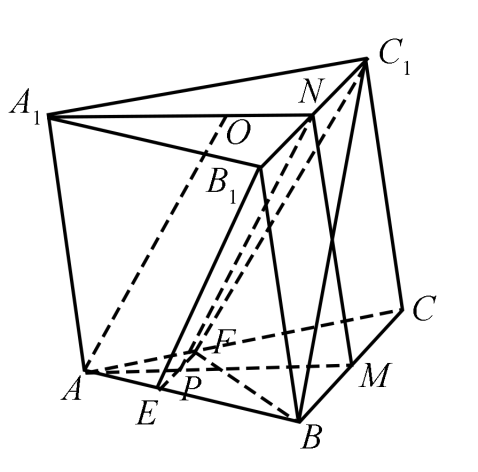
\includegraphics[width=\linewidth]{figures/2020_xkb2_wen_image53.png}\end{minipage}
\item（12分）

已知函数\emph{f}（\emph{x}）=2ln\emph{x}+1．

（1）若\emph{f}（\emph{x}）\ensuremath{\leq}2\emph{x}+\emph{c}，求\emph{c}的取值范围；

（2）设\emph{a}>0时，讨论函数\emph{g}（\emph{x}）=$\dfrac{f(x)-f(a)}{x-a}$的单调性．


{{[}选修4---4：坐标系与参数方程{]}}

\item（10分）

已知曲线\emph{C}$_{1}$，\emph{C}$_{2}$的参数方程分别为\emph{C}$_{1}$：$\{\begin{matrix}x=4\cos^2\theta，\\\end{matrix}y=4\sin^2\theta\}\{$（\emph{θ}为参数），\emph{C}$_{2}$：$\{\begin{matrix}x=t+\dfrac{1}{t},\\\end{matrix}y=t-\dfrac{1}{t}\}\{$（\emph{t}为参数）.

（1）将\emph{C}$_{1}$，\emph{C}$_{2}$的参数方程化为普通方程；

（2）以坐标原点为极点，\emph{x}轴正半轴为极轴建立极坐标系.设\emph{C}$_{1}$，\emph{C}$_{2}$的交点为\emph{P}，求圆心在极轴上，且经过极点和\emph{P}的圆的极坐标方程.

{{[}选修4---5：不等式选讲{]}}

\item（10分）

已知函数$f(x)=|x-a^{2}|+|x-2a+1|$.

（1）当$a=2$时，求不等式$f(x)⩾4$的解集；

（2）若$f(x)⩾4$，求\emph{a}的取值范围.
\end{examanswers}

\end{document}
